\documentclass{standalone}
\usepackage{tikz}

\usetikzlibrary{calc}


\begin{document}

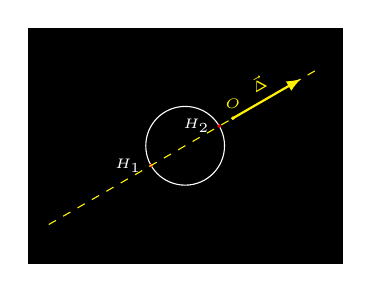
\begin{tikzpicture}
  \path[fill=black] (-2,-1.5) rectangle (2,1.5);
  \draw[white] (0,0) circle [radius=0.5cm];

  \coordinate (P1) at (210:0.5);
  \coordinate (P2) at (30:0.5);
  \coordinate (O) at ($ (P1) ! 1.2 ! (P2) $);

  \path[fill=red] (P1) circle [radius=0.025cm] node[left,font=\tiny,white] {$H_1$};
  \path[fill=red] (P2) circle [radius=0.025cm] node[left,font=\tiny,white] {$H_2$};

  \draw[dashed,yellow] ($ (P1) ! -1.5 ! (P2) $) -- ($ (P1) ! 2.5 ! (P2) $);
  \path[fill=yellow] (O) circle [radius=0.025cm] node[above,font=\tiny,yellow] {$O$};
  \draw[-latex,thick,yellow] (O) -- ($ (O) ! -1cm ! (P1) $) node[midway,above,sloped,font=\tiny] {$\vec\Delta$};
\end{tikzpicture}

\end{document}